\documentclass[a4paper, twoside, onecolumn, 10pt]{article}
% PACKAGES
\usepackage[utf8]{inputenc} % Usage des caractères spéciaux
\usepackage{fontenc}[T1]
\usepackage{enumerate} % Options supplémentaires pour les énumérations.
\usepackage[francais]{babel} % respect des normes françaises (table des matières etc...)
\usepackage{amsmath, amsfonts} % Packages mathématiques
\usepackage{graphicx} %insertion d'images dans LaTeX
\usepackage{blindtext} % texte aléatoire pour remplir
\blindmathtrue
\usepackage{geometry} % Géometrie de la page
\geometry{top    = 1.5cm, 
          bottom = 2cm, 
          left   = 3cm, 
          right  = 1cm}
\usepackage{verbatim}
\usepackage{booktabs} % To thicken table lines
\usepackage{array}
\usepackage[round]{natbib}
\usepackage{hyperref} % Liens hypertexte dans le document et index
\hypersetup{
    bookmarks=true,         % show bookmarks bar?
    unicode=false,          % non-Latin characters in Acrobat’s bookmarks
    pdftoolbar=true,        % show Acrobat’s toolbar?
    pdfmenubar=true,        % show Acrobat’s menu?
    pdffitwindow=false,     % window fit to page when opened
    pdfstartview={FitH},    % fits the width of the page to the window
    pdftitle={My title},    % title
    pdfauthor={Author},     % author
    pdfsubject={Les animaux aquatiques},   % subject of the document
    pdfcreator={SISEO},   % creator of the document
    pdfproducer={SISEO}, % producer of the document
    pdfkeywords={keyword1, key2, key3}, % list of keywords
    pdfnewwindow=true,      % links in new PDF window
    colorlinks=true,       % false: boxed links; true: colored links
    linkcolor=black,          % color of internal links (change box color with linkbordercolor)
    citecolor=green,        % color of links to bibliography
    filecolor=magenta,      % color of file links
    urlcolor=cyan           % color of external links
}

\usepackage{fancyhdr} % En tête et pieds de pages
\pagestyle{fancy}
\fancyhf{}
\fancyhead[LE,RO]{Formation \LaTeX SISEO 2018}
\fancyhead[RE,LO]{\leftmark}
\fancyfoot[CE,CO]{\rightmark}
\fancyfoot[LE,RO]{\thepage}
\renewcommand{\headrulewidth}{2pt}
\renewcommand{\footrulewidth}{1pt}

% COMMANDS AND VARIABLES
\author{Ludovic}
\title{Une première prise en main de \LaTeX}
\date{Un jour en décembre}
%\setlength{\baselineskip}{2cm}

\begin{document}
%\onecolumn
\maketitle % titre


\tableofcontents % table des matières
%\twocolumn


\section{Une première partie} % Un titre de partie

\subsection{Une sous partie}

\subsubsection{Les énumérations}

\begin{itemize}
\item Une chose,
\item Une autre chose,
\item Une dernière chose.
\end{itemize}

\begin{enumerate}[i)]
\item Une chose,
\item Une autre chose,
\item Une dernière chose.
\end{enumerate}

\subsection{Les paragraphes}

%\noindent 
Du texte très intéressant mais aussi super profond qui veut dire des choses sur la vie en général mais aussi sur des cas particuliers. 
Du texte très intéressant mais aussi super profond qui veut dire des choses sur la vie en général mais aussi sur des cas particuliers.
Du texte très intéressant mais aussi super profond qui veut dire des choses sur la vie en général mais aussi sur des cas particuliers.
On aime les mots longs anticonstitutionellement anticonstitutionellement anticonstitutionellement anticonstitutionellement.
Enfin bon voila.

%\vspace{2cm} % espace vertical

Un nouveau paragraphe. 

\section{Les mathématiques avec \LaTeX}

Il existe deux grands types d'environnements de maths. des maths en ligne. Exemple, la fonction $f(\alpha) \geq 5$ . 

$$
f(\alpha) = \underbrace{
			   \sum_{i = 0}^\infty \zeta_{ik}^5
			          }_{=0}		          
$$

\begin{equation}
\frac{3}{2} \times \frac{4}{3} = 2 \Xi \mathcal E \mathcal R \mathbb R
\label{eq:fractions}
\end{equation}

On peut associer des labels aux équations et à tous les objets. Par exemple, on peut citer l'équation \ref{eq:fractions} qui est à la page \pageref{eq:fractions}.

\subsection{Matrices et autres environnements}

\begin{equation}
M = 
\begin{pmatrix}
a & \frac{2}{3} \\
\dfrac{5}{2} & 3/4 
\end{pmatrix}
\end{equation}

$$
a = \left(
	\dfrac{\alpha + \dfrac{\beta}{\kappa}}{5+\upsilon}                                                               
	\right)
$$


$$
f(x) = \left\lbrace 
       \begin{split}
       5 , \forall x \in \mathbb R^* \\
       12 \forall x \in \lbrace 0 \rbrace  
       \end{split}
       \right.
$$

\begin{eqnarray}
a & = &  b + c \\
  & \neq & d + z
\end{eqnarray}

\section{Commandes}
\newcommand{\myvec}[1]{\vec{ \underline{\underline{#1}}} } % Une commande perso
\newcommand{\myvecc}[3]{ (#1, #2, #3) } % Une commande perso

Par exemple, on veut afficher des vecteurs comme $ \myvec v$ ou encore $\myvec{AB}$. Et aussi $\myvecc{1}{2}{3}$  et $\myvecc 456$

\newcommand{\labelledmatrix}[1]{\begin{equation}
\begin{Bmatrix}
1 & 0\\
0 & 1 \\
\end{Bmatrix}
\end{equation}
\label{#1}}

\labelledmatrix{truc}

La matrice indentité \ref{truc}.
\section{Figures et graphiques}


On peut inclure des ragondins (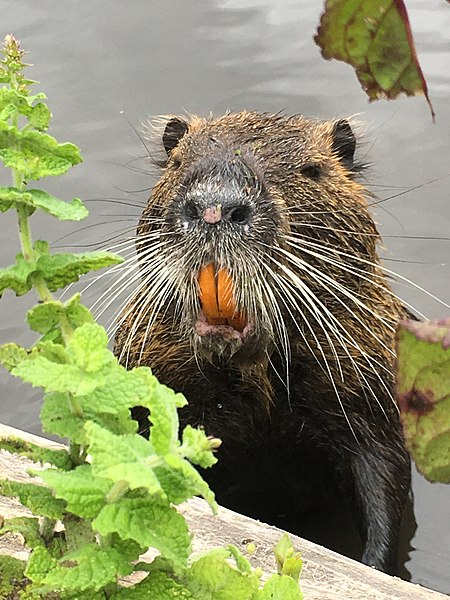
\includegraphics[scale=.1]{images/ragondin.jpg}) dans du texte !

\blindtext[10]

\begin{figure}[tb!]
\begin{center}
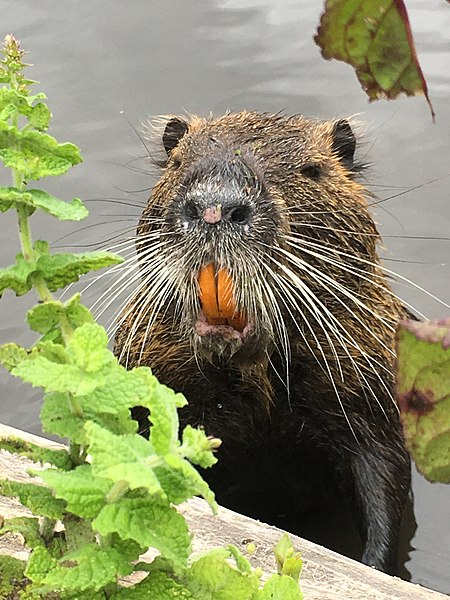
\includegraphics[width = .9\columnwidth]{images/ragondin.jpg}
\end{center}
\caption{L'invasion des ragondins. L'invasion des ragondins. L'invasion des ragondins. L'invasion des ragondins. L'invasion des ragondins. L'invasion des ragondins. L'invasion des ragondins. L'invasion des ragondins. L'invasion des ragondins. L'invasion des ragondins. L'invasion des ragondins. L'invasion des ragondins. L'invasion des ragondins. L'invasion des ragondins. L'invasion des ragondins. L'invasion des ragondins. L'invasion des ragondins. L'invasion des ragondins. L'invasion des ragondins. }
\label{fig:ragondin}
\end{figure}

\begin{figure}[tb!]
\begin{center}
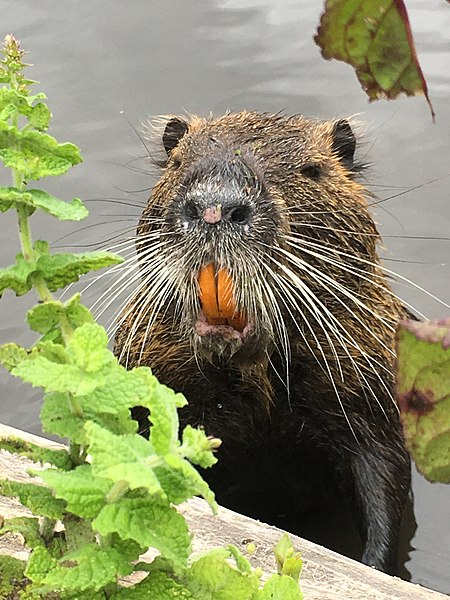
\includegraphics[width = .4\textwidth]{images/ragondin.jpg}
\end{center}
\caption{Ils sont de retour !  Ils sont de retour ! Ils sont de retour ! Ils sont de retour ! Ils sont de retour ! Ils sont de retour ! Ils sont de retour ! Ils sont de retour ! Ils sont de retour ! Ils sont de retour ! Ils sont de retour ! Ils sont de retour ! Ils sont de retour ! Ils sont de retour ! }
\label{fig:ragondin2}
\end{figure}

\begin{figure*}[h]
\begin{center}
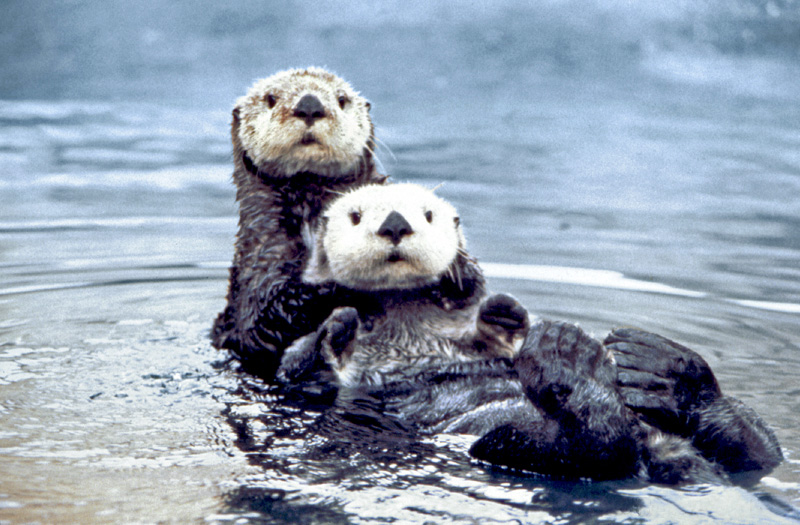
\includegraphics[width = .9\textwidth]{images/loutre.jpg}
\end{center}
\caption{La loutre de mer. }
\label{fig:loutre}
\end{figure*}


\blindtext[20]

\section{Tabular \& Table}

\subsection{Objet tabulaire non flottant avec Tabular}

\blindtext[2]

\begin{tabular}{l|cr}
\hline
truc & machin & bidule \\
\hline
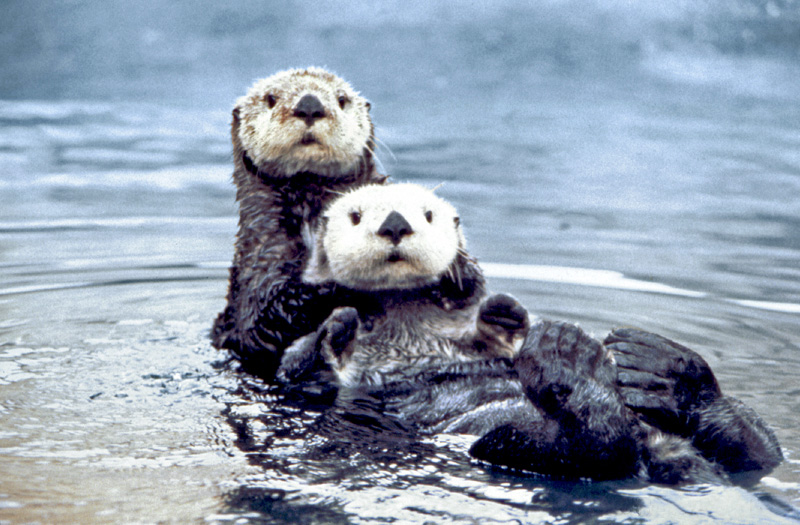
\includegraphics[scale = .03]{images/loutre.jpg} & $32 = \infty$ & $0 =0$\\
\hline
\end{tabular}

Une table créé avec Python.

\begin{table}
\begin{center}
\begin{tabular}{lccc}
\toprule
{} &         \textbf{A} &         \textbf{B} &         \textbf{C} \\
\midrule
0 &  0.250636 &  0.823901 &  0.439300 \\
1 &  0.860391 &  0.429316 &  0.067697 \\
2 &  0.189795 &  0.995844 &  0.917498 \\
3 &  0.559900 &  0.941000 &  0.296902 \\
4 &  0.138841 &  0.734202 &  0.902417 \\
5 &  0.255318 &  0.053967 &  0.622392 \\
6 &  0.383422 &  0.823361 &  0.987245 \\
7 &  0.710030 &  0.006286 &  0.793377 \\
8 &  0.362961 &  0.976675 &  0.322662 \\
9 &  0.509669 &  0.471906 &  0.092477 \\
\bottomrule
\end{tabular}
\end{center}
\caption{Une table !}
\label{tab:une_table}
\end{table}

\subsection{Usage du package array}

%\usepackage{array} %A ajouter
\begin{tabular}{c|m{7.cm}}
3 & In my opinion, it is a bug and should be reported. Tweak for the impatient: add one extra column with zero width and no padding.  \\
4 & In my opinion, it is a bug and should be reported. Tweak for the impatient: add one extra column with zero width and no padding.  \\
\end{tabular}


\blindtext[2]

\section{Bibliographie avec BibTex}
% Penser a importer aussi \usepackage{natbib} pour utiliser \citet et \

On peut citer les travaux de \citet{ferrets_rats}. Il a été démontré que les furets sont nombreux \citep{PMID2899444} et que ce nombre est en hausse. 

% BIBLIOGRAPHIE
\bibliographystyle{apalike}
\bibliography{biblio} % Chemin relatif vers le fichier biblio.bib (ne pas mettre le '.bib' dans le chemin)

\section{Packages utiles}
% \usepackage{hyperref} % Liens hypertexte dans le document et index


\end{document}